\section{Introduction}
\label{sec:introduction}

% General introduction
This tutorial helps you learn to use PFunc, short for Parallel Functions, a
lightweight and portable library that provides C and \Cpp{} APIs to express
task parallelism. 
%
PFunc enables programmers to focus on developing parallel algorithms and
specify low-level and high-level tasks to parallelize instead of working with
native threading libraries such as POSIX and Windows threads.
%
Although there are several task libraries, PFunc is unique in that its features
are a strict superset of the features offered by current solutions for task
parallelism.  
%
Specifically, PFunc extends the feature set of current solutions with custom
task scheduling, task priorities and task affinities.
%
In addition, PFunc offers task groups for SPMD-style programming and multiple
task completion notifications for parallel execution of DAGs. 
%
PFunc's extended feature set is geared towards helping knowledgeable users
optimize their application performance. 
%

\subsection{Organization}
\label{subsec:organization}
%
\begin{figure}[t]
\centering
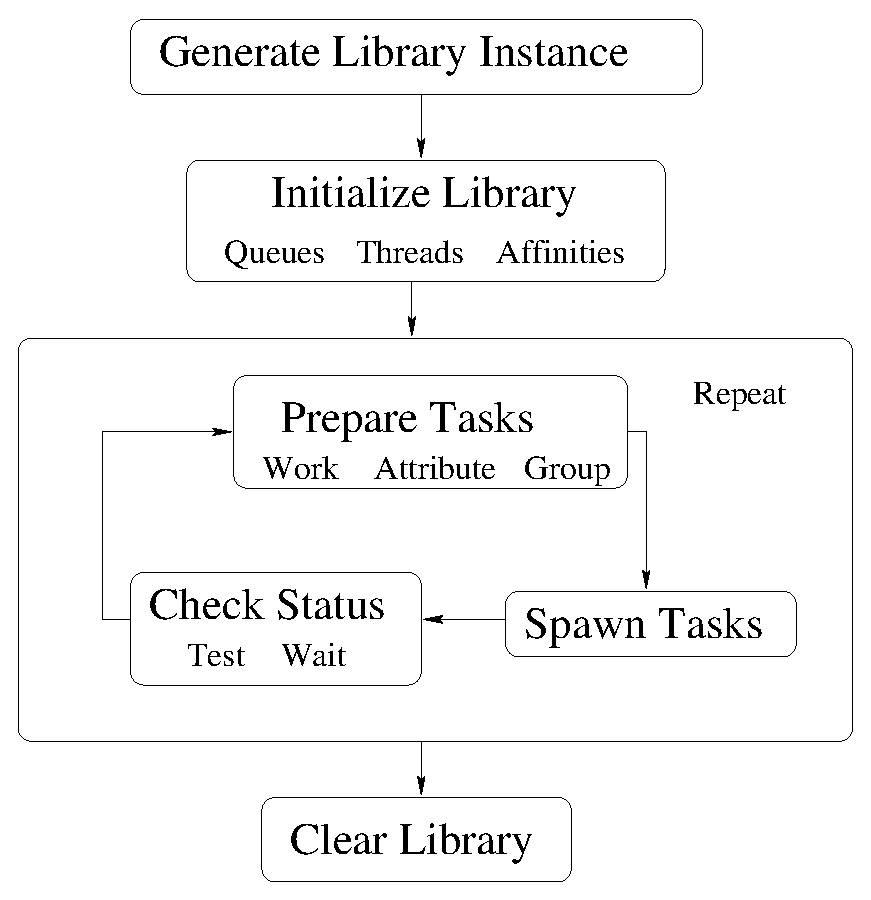
\includegraphics[width=0.5\textwidth]{figs/life-cycle}
\caption{Life-cycle of a PFunc application.}
\label{fig:life_cycle}
\end{figure}
%
Figure~\ref{fig:life_cycle} depicts the life-cycle of a PFunc
application. 
%
First, the library is initialized. Then, tasks are repeatedly spawned and
executed in parallel.  Finally, the library instance is cleared.
%
This tutorial is organized to reflect the life-cycle of PFunc applications.
 
\begin{center}
\begin{tabular}{|c|l|}
\hline
Section & Explanation \\
\hline
Section~\ref{sec:introduction} & Introduction to the tutorial.\\
\hline
Section~\ref{sec:install} & Installation and package information.\\
\hline
Section~\ref{sec:generate} & Generating PFunc's library instance description.\\
\hline
Section~\ref{sec:initialize} & Initializing the library.\\
\hline
\end{tabular}
\end{center}
